\documentclass[12pt]{article}

\usepackage{sbc-template}
\usepackage{subfigure} 
\usepackage{float} 
\usepackage{graphicx,url}
\usepackage[brazil]{babel}   
%\usepackage[latin1]{inputenc}  
\usepackage[utf8]{inputenc}  
% UTF-8 encoding is recommended by ShareLaTex

     
\sloppy

\title{Angular 2/4 Conceitos Básicos}

\author{Rafael Gonçalves de Oliveira Viana\inst{1} }


\address{Sistemas de Informação -- Universidade Federal do Mato Grosso do Sul
	(UFMS)\\
  	Caixa Postal 79400-000 -- Coxim -- MS -- Brazil
  \email{rafael.viana@aluno.ufms.br}
}

\begin{document} 

\maketitle

\begin{abstract}
This article describes how to build an Angular 2/4 application, use Angular-CLI, which allows administration of application components, offering better performance and speed in the production of Front End APIs.
\end{abstract}
     
\begin{resumo} 
  Este artigo descreve como iniciar uma aplicação Angular 2/4, utilizando o Angular-CLI, que permite administar os componentes da apliacação práticamente, tendo um melhor desempenho e velocidade na produção de APIs Front-End. 
\end{resumo}


\section{Introdução}

Angular 2 é uma estrutura mais eficiente que permite que os programadores se concentrem apenas na criação de classes de JavaScript. As visualizações e controladores do Angular 1.x são substituídos por componentes, que podem ser descritos como uma versão refinada de diretrizes.

Até mesmo os programadores angulares experientes nem sempre estão conscientes de todas as capacidades das diretivas Angular 1.x. Os componentes Angular 2 são consideravelmente mais fáceis de ler, e sua API possui menos jargão do que as diretrizes Angular 1.x.

A nova base de código angular é mais moderna, mais capaz e mais fácil para os novos programadores aprender do que Angular 1.x, ao mesmo tempo em que é mais fácil para os veteranos de projetos trabalharem.

Com o Angular 1, os programadores tiveram que entender as diferenças entre controladores, serviços, fábricas, fornecedores e outros conceitos que poderiam ser confusos, especialmente para novos programadores.

Apesar de ser uma reescrita completa, o Angular 2 manteve muitos dos seus principais conceitos e convenções com Angular 1.x, por exemplo, uma implementação simplificada, de injeção de dependência \cite{ehrenfeucht1992angular}, na Figura \ref{fig:De} é demostrado o desempenho do Angular 2.x em comparação com Angular 1.x. 

\begin{figure}[H]
	\centering
	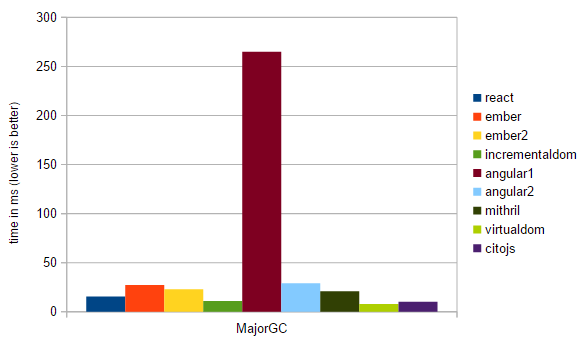
\includegraphics[width=0.5\textwidth]{imagens/desempenho.png}
	\caption{Desempenho Angular 2/4 X Angular 1, forncido pelo Auth0. }
	\label{fig:De}
	
\end{figure}



\subsection{Estrutura Angular 2/4}

O framework Angular consiste em várias bibliotecas, algumas delas básicas e algumas opcionais.
A estrutura é dividida em Modulos, Componentes, Serviços, Diretivas, Rotas.  
Ao escrever aplicativos compostos por modelos HTML com marcação \textit{angularizada}, escrevendo classes de componentes para gerenciar esses modelos criados, adicionando lógica. Em seguida, você inicia o aplicativo iniciando o módulo raiz. O Angular apresenta o conteúdo da sua aplicação em um navegador e responde às interações do usuário de acordo com as instruções que você forneceu, entretanto, há mais do que isso, um exemplo de estrutura utilizada e mostrada na figura \ref{fig:Est}.


\begin{figure}[H]
	\centering
	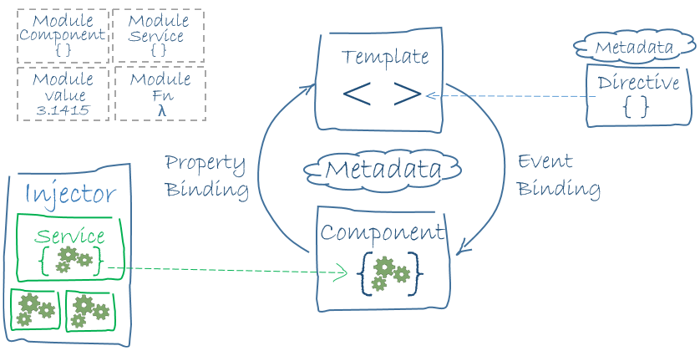
\includegraphics[width=0.5\textwidth]{imagens/EstruturaAngular.png}
	\caption{Estrutura Angular.}
	\label{fig:Est}
	
\end{figure}



\subsection{Angular 2/4}
	Para aqueles que pensam que ouve grandes mudanças da versão 2 para a 4, fiquem sabendo que foi apenas algumas caracteristicas que mudaram, não ouve a rescrita do código do Angular, como aconteceu na versão 1.x para 2.x.
	
	No Angular 2, a equipe introduziu a \textit{Semantic Versioning}, que nada mais nada menos faz com que atribui uma versão de 3 números a uma nova versão:\textbf{Major}, \textbf{Minor},\textbf{Patch}.\cite{codeangular}
	
	E no caso do Angular 4, a equipe usou a especificação de versionamento semântico, ou mais conhecido como: \textit{SemVer}.
	Se você sabe Angular 2 , não mudou em nada com a nova versão 4, as mudanças visão a integridade do código, evitando que em futuras modificações o código se quebre, assim como o engenheiro da Google Igor Minar disse:
	\begin{quote}
		\textit{“Queremos evitar quebras de ruptura nos códigos, assim como aconteceu com Angular 1.x para 2.x!”}
	\end{quote}


\subsection{title}
\section{TypeScript} \label{sec:firstpage}

Angular 2 foi escrito em TypeScript, um superconjunto de JavaScript que implementa muitos novos recursos ES2016 +.
Ao se concentrar em tornar a estrutura mais fácil para os computadores processarem, Angular 2 permite um ecossistema de desenvolvimento muito mais rico.

Os programadores que usam editores de texto sofisticados (ou IDEs) notarão melhorias dramáticas com auto-complete e sugestões de tipo. Essas melhorias ajudam a reduzir o ônus cognitivo da aprendizagem Angular 2. Felizmente para os programadores JavaScript tradicionais do ES5 isso não significa que o desenvolvimento deve ser feito em TypeScript ou ES2015: os programadores ainda podem escrever o JavaScript vanila que funciona sem transpilação.

Uma vez que a maioria dos navegadores não estão habilitados para rodar ES6 e ES7, surgiram alguns pré-compiladores, que geram todo o código para o JavaScript “entendível” pelo navegador. Mas o Typescript vai um pouco mais longe.

O TypeScript, criado pela Microsoft, é um “\_superset\_” do JavaScript, que, além de implementar as funcionalidades do ES6+, traz uma série de “poderes” no desenvolvimento. A capacidade de autocomplete nas IDEs é impressionante. Mas o mais interessante é a parte de organização do código. O TypeScript tem uma sintaxe muito mais clara e fácil de entender.

A primeira iteração da Angular forneceu programadores web com uma estrutura altamente flexível para o desenvolvimento de aplicativos. Esta foi uma mudança dramática para muitos programadores da web, e enquanto essa estrutura era útil, tornou-se evidente que muitas vezes era muito flexível. Ao longo do tempo, as melhores práticas evoluíram, e uma estrutura orientada pela comunidade foi endossada.

Angular 1.x tentou trabalhar em torno de várias limitações do navegador relacionadas ao JavaScript. Isto foi feito através da introdução de um sistema de módulos que utilizou a injeção de dependência. Este sistema era novo, mas infelizmente tinha problemas com as ferramentas, como na minificação e análise estática.

O Angular 2.x utiliza o sistema do módulo ES2015 e as modernas ferramentas de embalagem como o webpack, SystemJS e atualmente o Angular-CLI. Os módulos são muito menos acoplados ao "caminho angular", e é mais fácil escrever JavaScript mais genérico e conectá-lo ao Angular. A remoção de soluções alternativas de minificação e a adição de prescrições rígidas tornam a manutenção das aplicações existentes mais simples. O novo sistema de módulos também facilita o desenvolvimento de ferramentas eficazes que podem justificar melhor os projetos maiores.\cite{bierman2014understanding}

\section{Mobile}

Angular 2 foi projetado para o celular desde do seu início. Além do poder de processamento limitado, os dispositivos móveis possuem outros recursos e limitações que os separam dos computadores tradicionais. As interfaces de toque, as propriedades de tela limitada por esse motivo o hardware móvel foram considerados no Angular 2.
Os computadores de mesa também tiverão melhorias dramáticas no desempenho e na capacidade de resposta.
O Angular 2, como React e outras estruturas modernas, pode aproveitar os ganhos de desempenho ao renderizar HTML no servidor ou mesmo em um trabalhador da Web. A busca pelo desempenho não termina com pré-renderização. O Angular 2 torna-se portátil para o celular nativo, integrando-se ao NativeScript, uma biblioteca de código aberto que engata o JavaScript e o celular. Além disso, a equipe Ionic está trabalhando em uma versão Angular 2 de seu produto, fornecendo outra maneira de alavancar recursos nativos dos dispositivos com Angular 2.

Se você pretende desenvolver aplicativos híbridos, cá está mais um excelente motivo para usar Angular 2, a equipe do Ionic está finalizando o desenvolvimento da sua segunda versão, que é totalmente escrita em Angular 2.

\section{Node JS}
Node.js é uma plataforma para desenvolvimento de aplicações server-side baseada no V8, o interpretador de JavaScript open source implementado pelo Google em C++ e utilizado pelo Chrome. O que sem dúvidas gera uma grande expectativa em relação ao desempenho do Node.js. Sendo assim utilizando JavaScript e o interpretador V8 JavaScript podemos criar uma variedade de aplicações Web utilizando apenas código em JavaScript.


\section{Angular Cli}
Iniciar e gerenciar um projeto em Angular 2 pode não ser uma tarefa tão simples. A existência de dezenas de bibliotecas, frameworks e ferramentas, que muitas vezes tentam resolver o mesmo problema, pode ser uma barreira aos primeiros contatos com a tecnologia.

Ao observar esse problema, a equipe do Angular criou uma ferramenta de linha de comando chamada Angular CLI (Command Line Interface - Interface de Linha de Comando) cujo objetivo principal é facilitar o gerenciamento de projetos escritos nesse framework.

Existe uma lista de comandos Angular CLI, esses podem ser encontrados na página do mesmo em: wwww.cli.angular.io, porém para fins didatico ser mostrado apenas os comandos para inicialização "ng new " e desenvolvimento "ng server" 

Com o Node.JS instalado, temos à disposição o comando npm, necessário para instalar o Angular CLI. Neste ponto, será preciso abrir o terminal do seu sistema operacional e digitar a instrução:
\begin{verbatim}
	                                  npm install -g @angular/cli
\end{verbatim}

Após a instalação pode-se ver, se esta tudo correto executando o comando:

\begin{verbatim}
                                             ng help
\end{verbatim}

Se estiver tudo correto será mostrado uma lista de comando disponíveis pelo Angular CLI, sendo assim pode-se começar a trabalhar com o Angular 2, basta cria um projeto com o comando de inicialização do Angular-CLI: 


\begin{verbatim}
                                       ng new nomedoprojeto
\end{verbatim}

Após a criação do projeto com o comando de inicialização do Angular CLI demostrado na Figura \ref{fig1}, terá um projeto, "Hello World" como na Figura \ref{fig2} , pronto para ser executado:

\begin{figure}[H]
	\center
	\caption{}
	\subfigure[Construindo\label{fig1}]{
	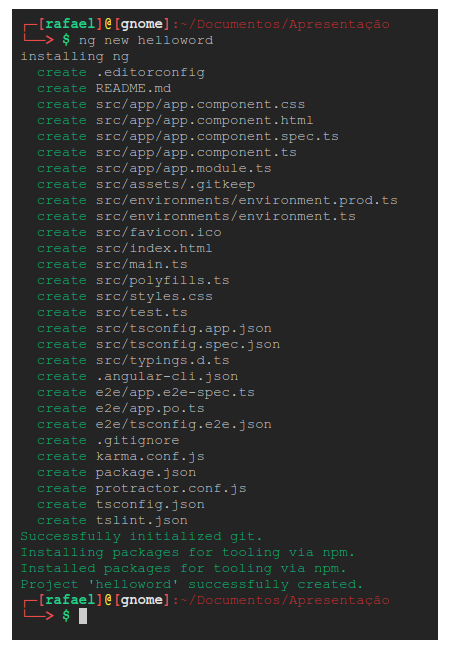
\includegraphics[width=6.8cm]{imagens/01.png}}
    \subfigure[Construído\label{fig2}]{
	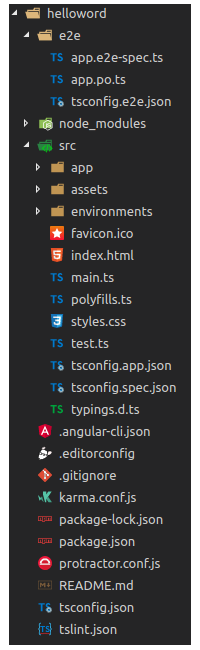
\includegraphics[width=3cm]{imagens/02.png}}
	\center
\end{figure}

Para poder roda o projeto em nível de desenvolvimento já dentro da pasta do projeto utiliza o comando: 
	\begin{verbatim}
	                                    ng server
	\end{verbatim}
	
O projeto será executado pela porta 4200 por padrão, abrindo um navegador web e entrando no caminho localhost:4200, pode ver o projeto rodando Figura \ref{fig:Esta}. 	


\begin{figure}[H]
	\centering
	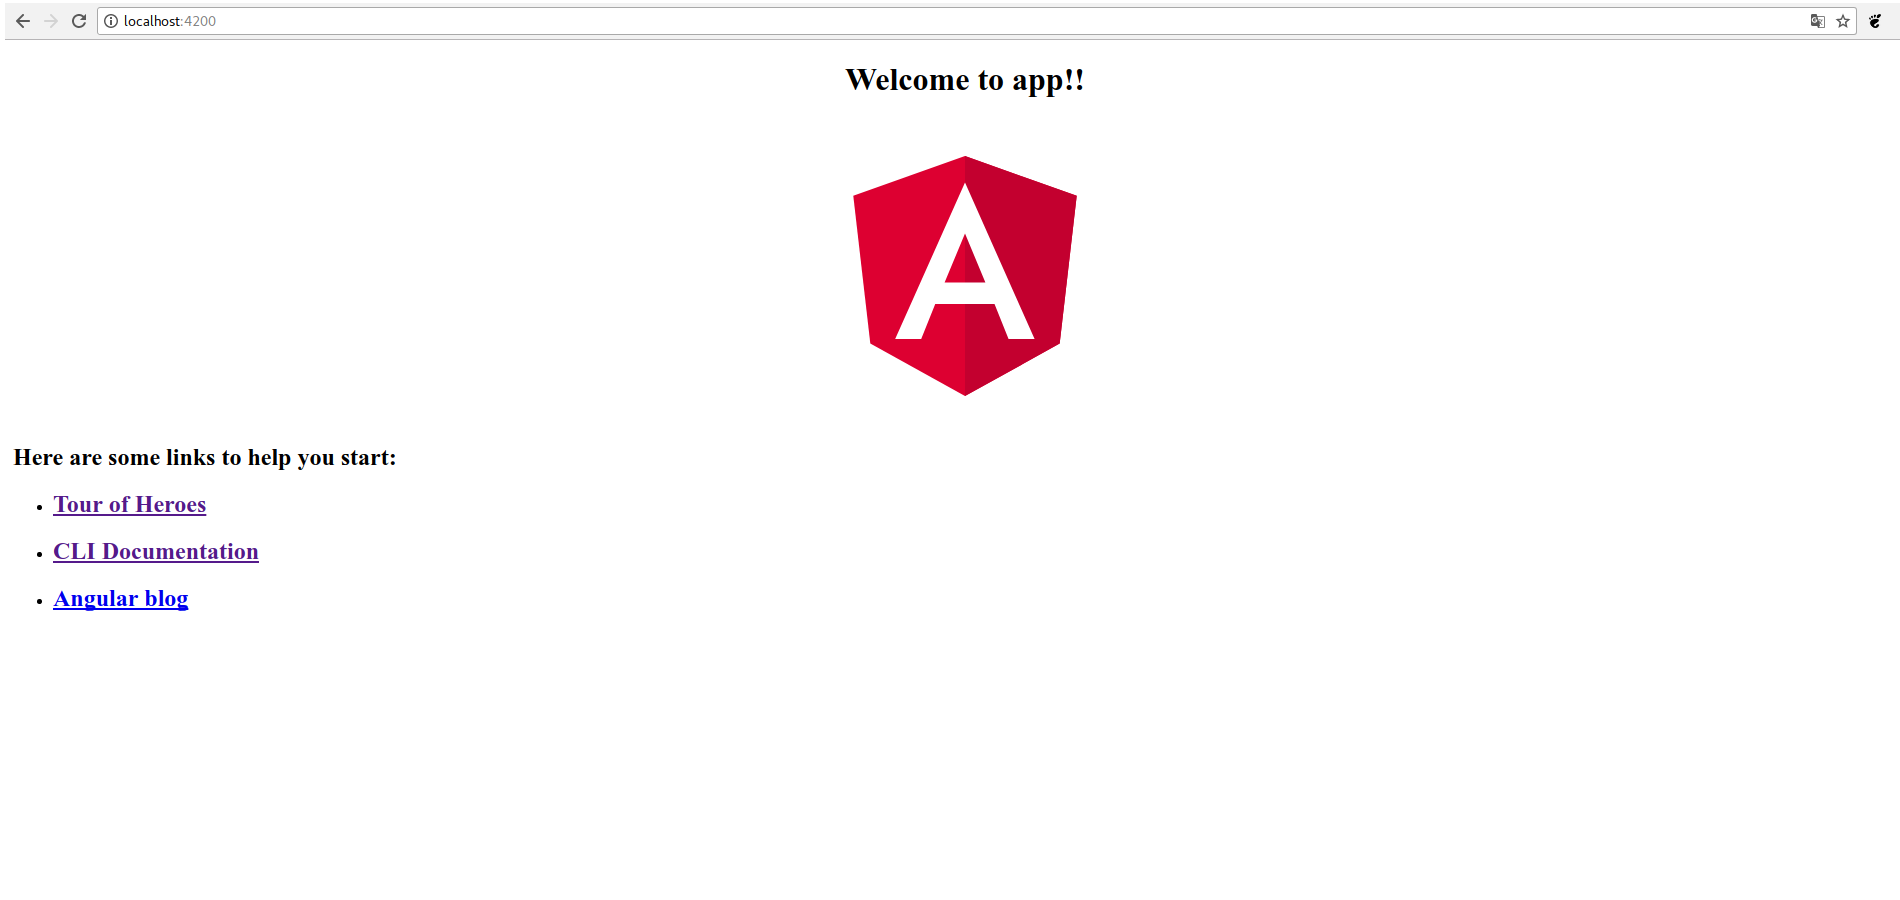
\includegraphics[width=0.8\textwidth]{imagens/Angula2.png}
	\caption{Projeto rodando.}
	\label{fig:Esta}
	
\end{figure}

\section*{Conclusão}

Para começar a aprender Angular 2/4 não precisa saber o Angular 1.x, já que a estrutura foi reescrita pelos engenheiros da Google, em uma estrutura que proporciona um melhor entendimento do código, sendo mais fácil a leitura e a codificação de aplicações, além da melhoria na estrutura o desempenho demostrado pelo Angular 2/4 foi muito superior em comparação com seu antecessor. Já para queles programadores que vem da versão 1.X, a curva de aprendizagem ainda é menor pelo domínio de alguns conceitos da versão 1.x ainda mantidos na versão 2/4. Sendo assim o Angular 2/4 deu um tremendo salto na frente da versão 1.x, em questão de velocidade de produção.
 
\bibliographystyle{sbc}
\bibliography{sbc-template}

\end{document}
